\documentclass{article} % For LaTeX2e
\usepackage{nips13submit_e,times}
\usepackage{hyperref}
\usepackage{float}
\usepackage{url}
\usepackage[pdftex]{graphicx} 
\usepackage{listings}
\usepackage{geometry}
%\documentstyle[nips13submit_09,times,art10]{article} % For LaTeX 2.09


\title{A Study of the Sleeping Situation of PSU students by  a Two-factor ANCOVA Experiment}


\author{
Jiarong Ye \\
College of Engineering\\
The Pennsylvania State University\\
State College, PA 16801 \\
\texttt{jxy225@psu.edu} \\
}


\newcommand{\fix}{\marginpar{FIX}}
\newcommand{\new}{\marginpar{NEW}}

\nipsfinalcopy 

\begin{document}


\maketitle

\begin{abstract}
The motivation of this report is to observe the sleeping situation of PSU students and study the relations between the average sleeping hours of students and influence factors including their class standing, majors, the interaction term of class standing and majors and the number of dues they have every week, which is considered the covariate in the experiment. The experimental units are PSU students including freshmen, sophomore, junior and senior majoring in Engineering, Business and Liberal Arts. And the data model applied to the experiment is the Two-Factor ANCOVA model.

\end{abstract}

\section{Introduction}



As students get heavier workload and higher stress level of students when the final month approaches, their sleeping condition is affected as well. And the effect differs for students in different class standing and majors. For example, compared with freshmen, seniors are more likely to take on a heavier workload and have more responsibilities such as academic research or job searching. And the majors students are in play an important role as well. Engineering students usually have more academic obligations such as experiments, labs, group projects, technical papers that they need  to work on. So are the students in the smeal college of business studying finance, accounting and marketing where case studies require lots of work. In comparison, Liberal Arts students might have a more flexible class schedule and not be as busy as their peers in Engineering and Business. Therefore in order to confirm this speculation, a Two-Factor ANCOVA Model is constructed to test the relations between the response (average sleeping hours per week), two factors (class standing and major) and one covariate (number of dues per week). 

\section{Data Set}
The dataset for the experiment is randomly collected from 60 full-time PSU students taking a bio-behavioral health general education class through informal surveys I conducted at the beginning of each class in November. The response from 48 students are used, among which 16 of them major in Engineering, 16 of them major in Business and 16 of them major in Liberal Arts in each class standing respectively (freshmen, sophomore, junior, senior). Their average sleeping hours and the total number of dues in that specific week are collected.
The attributes contained in the dataset include:
\begin{itemize}
\item  \textbf{Class standing}
\item  \textbf{Major}
\item  \textbf{Number of dues per week (covariate)}
\item  \textbf{Average sleeping hours per week}
\end{itemize}


%latex.default(df, out = "e.tex")%
\begin{table}[H]
	\begin{center}
		\begin{tabular}{|l|l|l|r|r|}
			\hline
			\multicolumn{1}{|l|}{df}&\multicolumn{1}{|c|}{class}&\multicolumn{1}{|c|}{major}&\multicolumn{1}{|c|}{num\_of\_dues\_per\_week}&\multicolumn{1}{|c|}{avg\_sleep\_hrs\_per\_week}\tabularnewline
			\hline
			1&freshmen&Engineering&$5$&$7.1$\tabularnewline
			2&freshmen&Engineering&$4$&$7.5$\tabularnewline
			3&freshmen&Engineering&$6$&$7.2$\tabularnewline
			4&freshmen&Engineering&$7$&$6.9$\tabularnewline
			5&freshmen&Business&$4$&$7.1$\tabularnewline
			6&freshmen&Business&$3$&$7.6$\tabularnewline
			7&freshmen&Business&$3$&$7.4$\tabularnewline
			8&freshmen&Business&$5$&$7.1$\tabularnewline
			9&freshmen&Liberal Arts&$2$&$8.5$\tabularnewline
			10&freshmen&Liberal Arts&$3$&$8.3$\tabularnewline
			11&freshmen&Liberal Arts&$4$&$8.0$\tabularnewline
			12&freshmen&Liberal Arts&$4$&$8.1$\tabularnewline
			13&sophomore&Engineering&$6$&$7.0$\tabularnewline
			14&sophomore&Engineering&$5$&$7.4$\tabularnewline
			15&sophomore&Engineering&$8$&$6.4$\tabularnewline
			16&sophomore&Engineering&$7$&$6.7$\tabularnewline
			17&sophomore&Business&$6$&$7.3$\tabularnewline
			18&sophomore&Business&$3$&$8.0$\tabularnewline
			19&sophomore&Business&$4$&$6.4$\tabularnewline
			20&sophomore&Business&$6$&$7.5$\tabularnewline
			21&sophomore&Liberal Arts&$4$&$8.0$\tabularnewline
			22&sophomore&Liberal Arts&$3$&$8.3$\tabularnewline
			23&sophomore&Liberal Arts&$3$&$8.2$\tabularnewline
			24&sophomore&Liberal Arts&$4$&$7.9$\tabularnewline
			25&junior&Engineering&$4$&$6.5$\tabularnewline
			26&junior&Engineering&$6$&$6.6$\tabularnewline
			27&junior&Engineering&$4$&$7.0$\tabularnewline
			28&junior&Engineering&$5$&$7.2$\tabularnewline
			29&junior&Business&$5$&$7.5$\tabularnewline
			30&junior&Business&$4$&$7.7$\tabularnewline
			31&junior&Business&$6$&$7.8$\tabularnewline
			32&junior&Business&$4$&$7.8$\tabularnewline
			33&junior&Liberal Arts&$4$&$7.1$\tabularnewline
			34&junior&Liberal Arts&$5$&$7.7$\tabularnewline
			35&junior&Liberal Arts&$5$&$7.8$\tabularnewline
			36&junior&Liberal Arts&$4$&$7.6$\tabularnewline
			37&senior&Engineering&$6$&$6.4$\tabularnewline
			38&senior&Engineering&$5$&$6.9$\tabularnewline
			39&senior&Engineering&$5$&$5.9$\tabularnewline
			\hline
	\end{tabular}\end{center}
\end{table}


%latex.default(df, out = "e.tex")%
\begin{table}[H]
	\begin{center}
		\begin{tabular}{|l|l|l|r|r|}
			\hline
			\multicolumn{1}{|l|}{df}&\multicolumn{1}{|c|}{class}&\multicolumn{1}{|c|}{major}&\multicolumn{1}{|c|}{num\_of\_dues\_per\_week}&\multicolumn{1}{|c|}{avg\_sleep\_hrs\_per\_week}\tabularnewline
			\hline
			40&senior&Engineering&$7$&$6.1$\tabularnewline
			41&senior&Business&$6$&$6.5$\tabularnewline
			42&senior&Business&$4$&$7.3$\tabularnewline
			43&senior&Business&$5$&$6.8$\tabularnewline
			44&senior&Business&$6$&$6.4$\tabularnewline
			45&senior&Liberal Arts&$4$&$7.4$\tabularnewline
			46&senior&Liberal Arts&$2$&$8.0$\tabularnewline
			47&senior&Liberal Arts&$3$&$7.3$\tabularnewline
			48&senior&Liberal Arts&$3$&$7.8$\tabularnewline
			\hline
			\end{tabular}\end{center}
			\end{table}


\section{Exploratory Data Analysis}

Next we look at the data multivariately with figures:
\subsection{Weekly Average Sleeping Hours}

\begin{figure}[H]
	\begin{center}
		%\framebox[4.0in]{$\;$}
		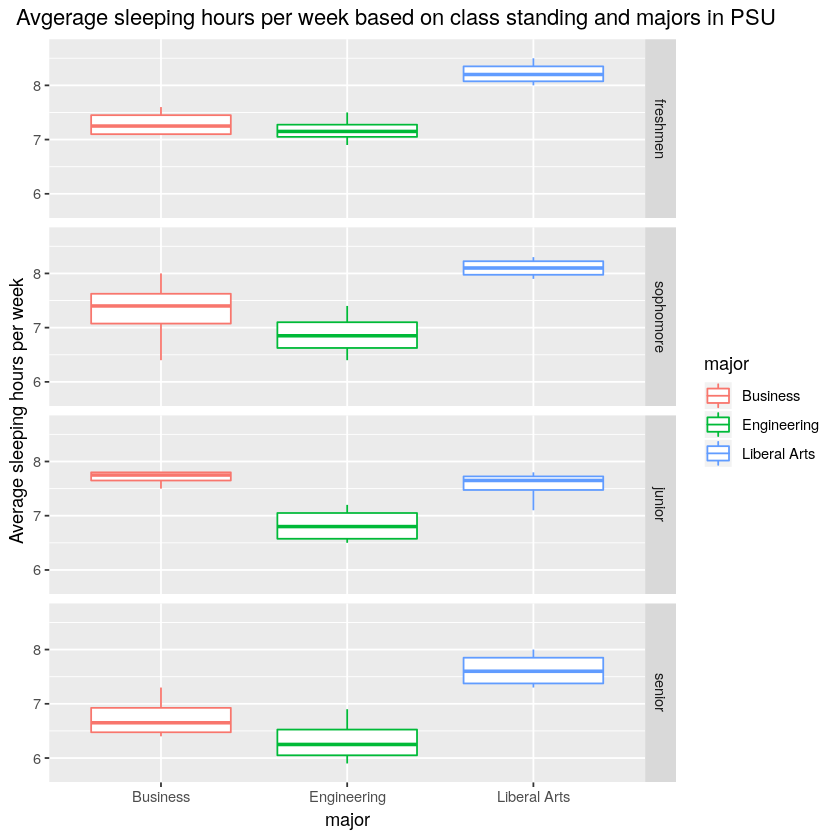
\includegraphics[height=8cm, width=11cm]{3.png}
	\end{center}
	\caption{Average sleeping hours per week of different majors}
\end{figure}

\begin{figure}[H]
	\begin{center}
		%\framebox[4.0in]{$\;$}
		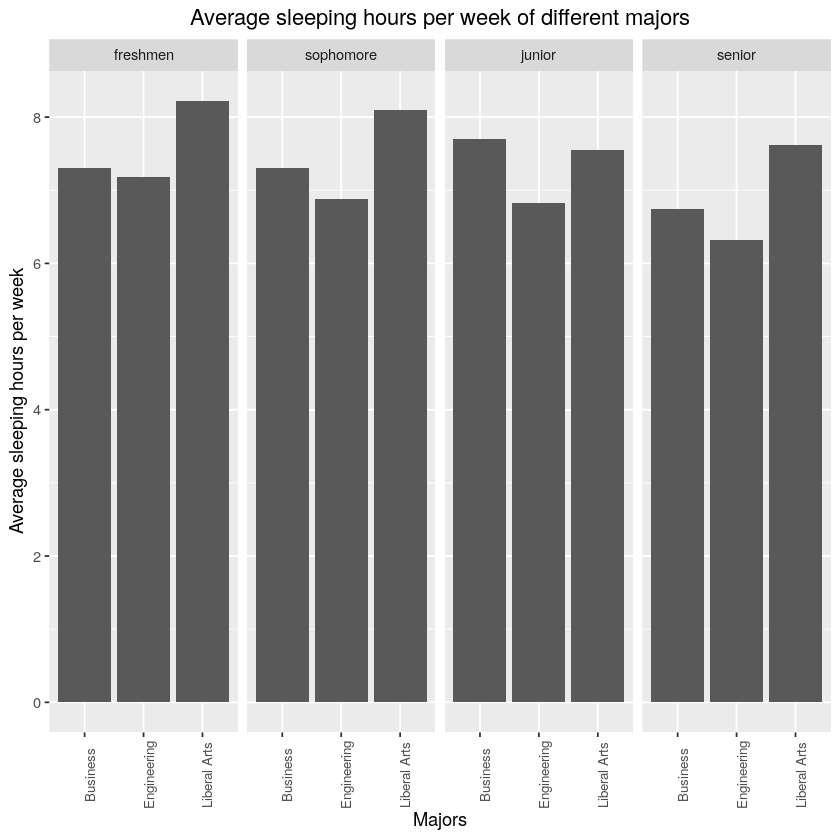
\includegraphics[height=6cm, width=10cm]{2.png}
	\end{center}
	\caption{Average sleeping hours per week of different majors}
\end{figure}




The apparent pattern we observe from the side-by-side bar plot as well as the boxplot is that Liberal Arts students get the longest sleeping hours from freshmen to senior, compared with students majoring in Engineering and Business. And the tendency as the class standing increases among all three majors is similar, freshmen obviously get more sleeping time than juniors and seniors.


\subsection{Weekly Number of Dues}

\begin{figure}[H]
	\begin{center}
		%\framebox[4.0in]{$\;$}
		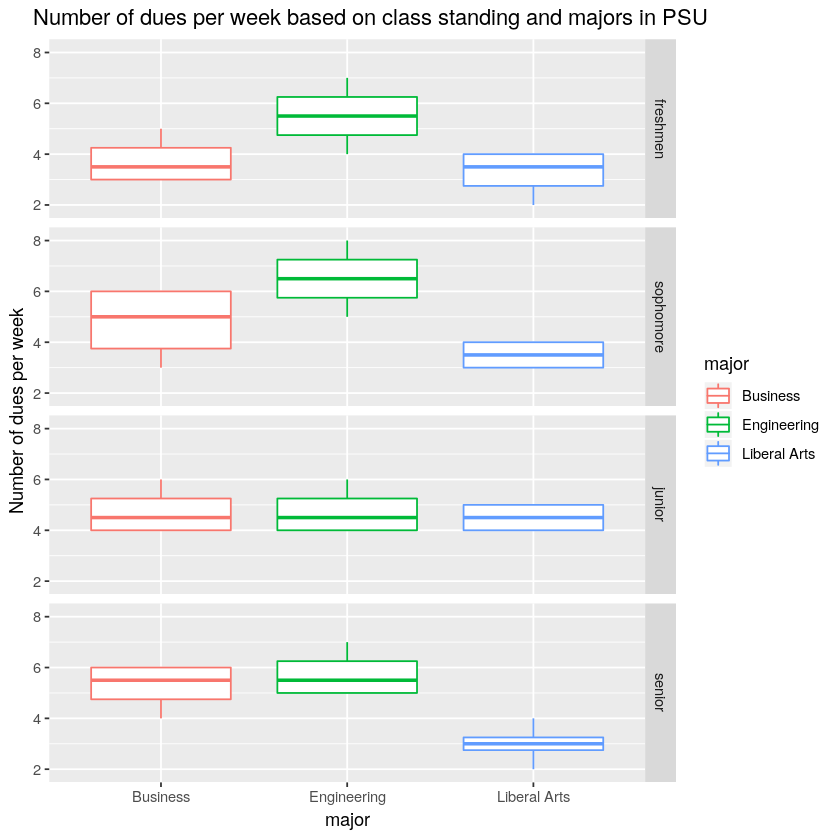
\includegraphics[height=8cm, width=10cm]{5.png}
	\end{center}
	\caption{Number of dues per week based on class standing and majors}
\end{figure}

\begin{figure}[H]
	\begin{center}
		%\framebox[4.0in]{$\;$}
		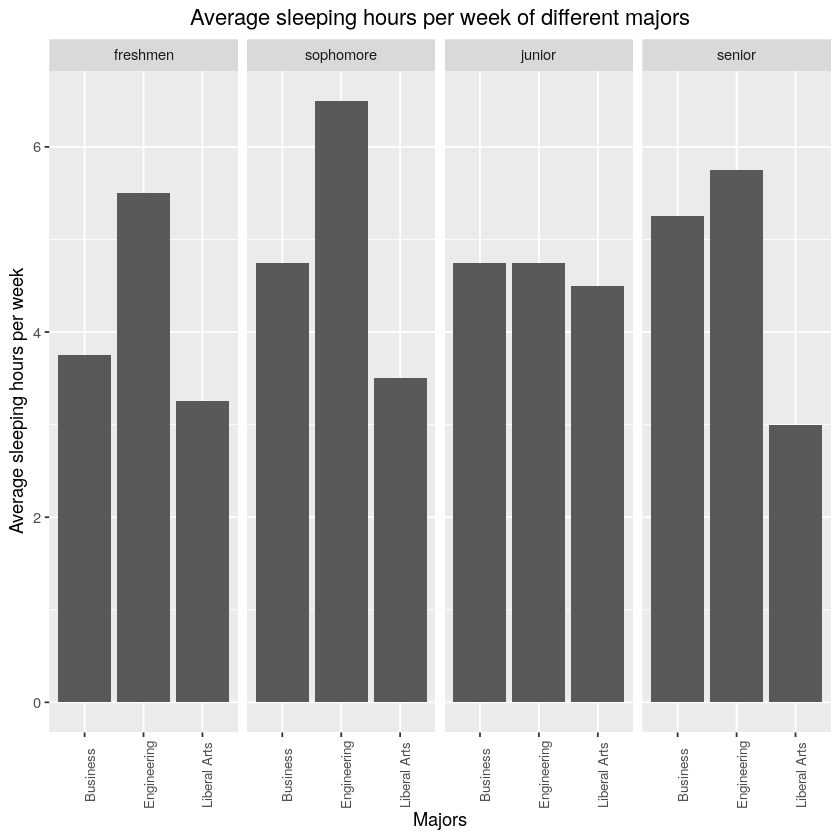
\includegraphics[height=6cm, width=10cm]{4.png}
	\end{center}
	\caption{Number of dues per week of different majors}
\end{figure}




Similar to the average sleeping hours, the number of dues per week share the same tendency that that Liberal Arts students have the least amount of workload from freshmen to senior, compared with students majoring in Engineering and Business. However unlike the relation of average sleeping hours and class standing presented in the figures above, the weekly dues number does not seem to differ significantly based on class standing.  

\section{Modeling}


\subsection{Description}

In the experiment, firstly, the hypothesis of linearity and equal slope assumption of the covariate will be tested in order to confirm the assumption is actually valid. secondly, the hypothesis regarding the significance of the interaction term (class\_standing:major) will be tested, if it is proven to be significant, then the pairwise differences between the combination of class\_standing and major are tested to determine how the interactive term is significant; if proven to be not significant, then the interaction term is drop and pairwise differences of single factor (class\_standing and major, respectively) will be tested.


\subsection{Data Model}

The Two-factor covariance data model for this experiment is:

$$Y_{ijt} = \mu + \alpha_{i} + \beta_{j} + (\alpha \beta)_{ij} + \gamma (X_{ijt} -\bar X_{...}) + \epsilon_{ijt}, \:\: \epsilon_{ijt}
\stackrel{iid}{\sim} N(0, \sigma^2)$$

\(\alpha\): The fixed effect of the factor class Standing (Freshmen, Sophomore, Junior, Senior) \\
$\beta$:  Major (Engineering, Business, Liberal Arts) \\
$X$: The number of dues per week  \\
$Y$: The average sleeping hours per week \\
$i = 1, 2, 3, 4, j = 1, 2, 3, t = 1, 2, 3, 4$ \\


\subsection{Analysis Before Model Building}
\subsubsection{Test of Interactions Between Factor and Covariate}


\textbf{1. The interaction between \textit{class standing} and \textit{number of dues per week}}

\begin{itemize}

\item 1. ANOVA(I(x -mean(x)) + class)

\item 2. ANOVA(I(x-mean(x))*class)

\end{itemize}

\begin{table}[H]
	\begin{center}
		\begin{tabular}{|l|r|r|r|r|r|r|}
			\hline\hline
			\multicolumn{1}{|l|}{anova}&\multicolumn{1}{|c|}{Res.Df}&\multicolumn{1}{|c|}{RSS}&\multicolumn{1}{|c|}{Df}&\multicolumn{1}{|c|}{Sum of Sq}&\multicolumn{1}{|c|}{F}&\multicolumn{1}{|c|}{Pr(\textgreater F)}\tabularnewline
			\hline
			1&$43$&$7.94571416749420$&$$&$$&$$&$$\tabularnewline
			\hline
			2&$40$&$7.02215422440894$&$
			 3$&$0.923559943085267$&$1.75361180927449$&$0.171576450358816$\tabularnewline
			\hline
	\end{tabular}\end{center}
\end{table}

\textbf{2. The interaction between major and number of dues per week}

\begin{itemize}
	
	\item 1. ANOVA(I(x -mean(x)) + major)
	
	\item 2. ANOVA(I(x-mean(x))*major)
	
\end{itemize}

\begin{table}[H]
	\begin{center}
		\begin{tabular}{|l|r|r|r|r|r|r|}
			\hline\hline
			\multicolumn{1}{|l|}{anova}&\multicolumn{1}{|c|}{Res.Df}&\multicolumn{1}{|c|}{RSS}&\multicolumn{1}{|c|}{Df}&\multicolumn{1}{|c|}{Sum of Sq}&\multicolumn{1}{|c|}{F}&\multicolumn{1}{|c|}{Pr(\textgreater F)}\tabularnewline
			\hline
			1&$44$&$7.83107894736842$&$$&$$&$$&$$\tabularnewline
			\hline
			2&$42$&$7.81652126882414$&$ 2$&$0.0145576785442874$&$0.0391109086658986$&$0.96167902939109$\tabularnewline
			\hline
	\end{tabular}\end{center}
\end{table}
We can observe from there ANOVA contrast table that after adding the interaction term \textbf{I(num\_of\_dues\_per\_week-mean(num\_of\_dues\_per\_week))*class} and \textbf{I(num\_of\_dues\_per\_week-mean(num\_of\_dues\_per\_week))*major} to the ANOVA model, the new $p$ value becomes $0.1715765$ which is $>0.05$ and  0.961679, which is also $>0.05$, indicating the additional interaction term between \textbf{num\_of\_dues\_per\_week} and \textbf{class standing} is not significant, and  the additional interaction term between \textbf{num\_of\_dues\_per\_week} and \textbf{major} is not significant either.

\subsubsection{Diagnostics of Linearity and Equal Slopes Assumptions}

\begin{figure}[H]
	\begin{center}
		%\framebox[4.0in]{$\;$}
		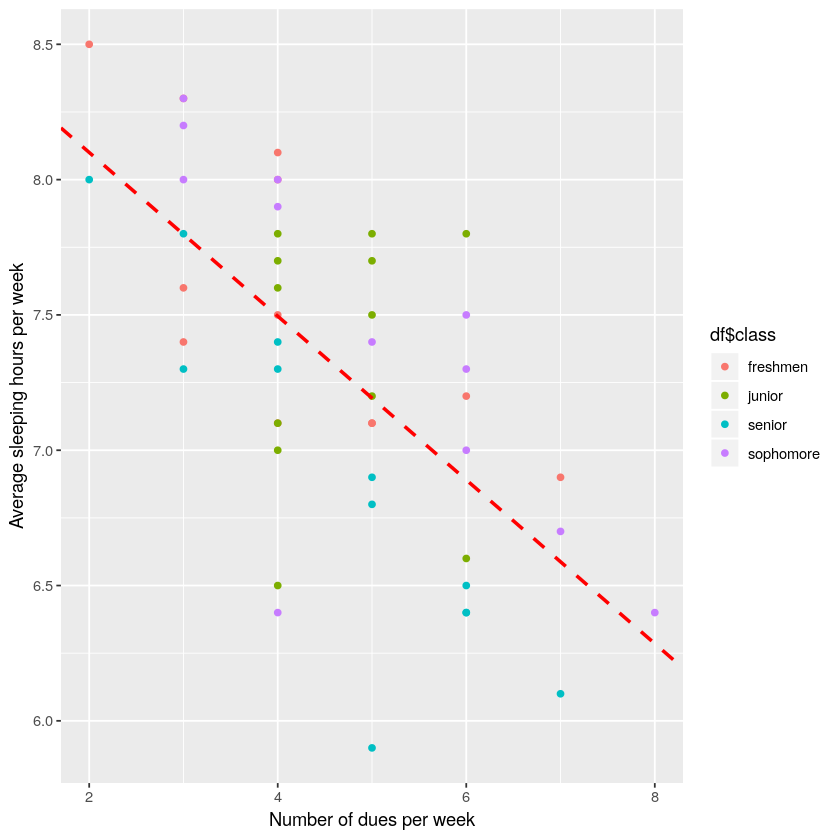
\includegraphics[height=8cm, width=10cm]{6.png}
	\end{center}
	\caption{Average sleeping hours per week vs. Number of dues per week}
\end{figure}


It appears that both the linearity and equal slopes assumptions required for
ANCOVA are valid. 

\subsection{ANCOVA Model}

\subsubsection{Interaction Term}

The first test is for the significance of  interaction terms:

\textbf{Null Hypothesis}:

$$H_0 : (\alpha \beta)_{ij} = 0 \:\:\: for \:\: all \:\:  i, j$$

\textbf{Alternative Hypothesis}:

$$H_a : (\alpha \beta)_{ij} \neq 0 \:\:\: for \:\: all \:\: i, j$$


\textbf{ANOVA Table:}

($note^*$ denote $x$: num\_of\_dues\_per\_week)
\begin{table}[H]
	\begin{center}
		\begin{tabular}{|l|r|r|r|r|r|}
			\hline\hline
			\multicolumn{1}{|l|}{anova}&\multicolumn{1}{|c|}{Df}&\multicolumn{1}{|c|}{Sum Sq}&\multicolumn{1}{|c|}{Mean Sq}&\multicolumn{1}{|c|}{F value}&\multicolumn{1}{|c|}{Pr(\textgreater F)}\tabularnewline
			\hline
			class&$ 3$&$2.99416666666667$&$0.998055555555556$&$ 9.81822073619254$&$7.68501150692738e-05$\tabularnewline
			major&$ 2$&$9.30500000000000$&$4.652499999999998$&$45.76826582535172$&$1.70770191448029e-10$\tabularnewline
			I(x - 
				mean(x))&$ 1$&$1.13158208020050$&$1.131582080200501$&$11.13176774848383$&$2.01977445976904e-03$\tabularnewline
			class:major&$ 6$&$1.56388212561606$&$0.260647020936010$&$ 2.56407568850839$&$3.64868969776764e-02$\tabularnewline
			Residuals&$35$&$3.55786912751677$&$0.101653403643336$&$$&$$\tabularnewline
			\hline
	\end{tabular}\end{center}
\end{table}


\textbf{Check Residuals Normality and Variance Constance Violation}


\begin{figure}[H]
	\begin{center}
		%\framebox[4.0in]{$\;$}
		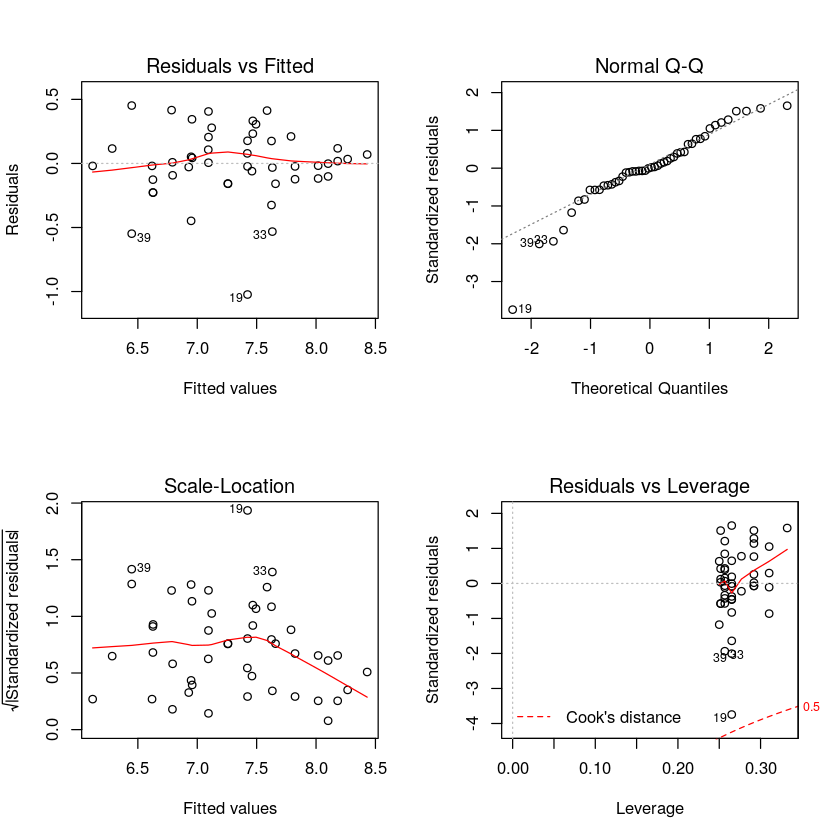
\includegraphics[height=8cm, width=10cm]{7.png}
	\end{center}
	\caption{Residual vs. Fitted Value Plot and QQ Plot}
\end{figure}

From the diagnostic plots above we can see that the assumptions of  normality and the constancy of variance of residuals are not violated. Therefore no transformation of variables is needed for this experiment.


 Therefore, from the ANCOVA table, we can see that the P value of \textbf{class:major} is 0.0364869, and since $0.0364869 < 0.05$, therefore under the significance level of $5\%$, we are confident enough to reject the null hypothesis and conclude that the interaction term is significant.
\newpage

\textbf{Confirm the significant interaction with interaction plot:}

\begin{figure}[H]
	\begin{center}
		%\framebox[4.0in]{$\;$}
		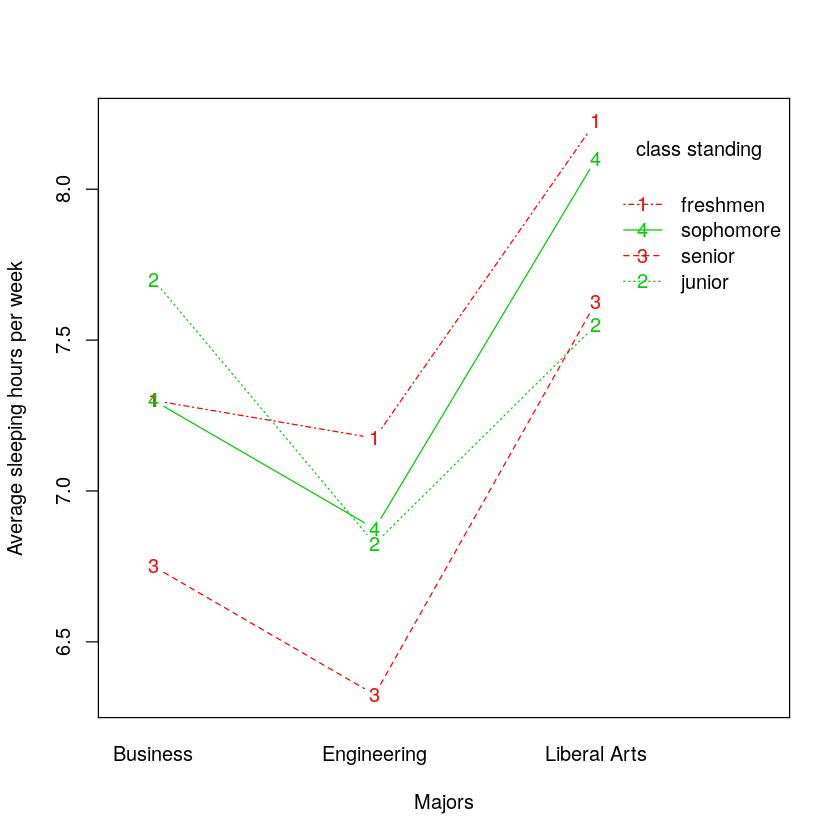
\includegraphics[height=8cm, width=10cm]{8.png}
	\end{center}
	\caption{Interaction Plot}
\end{figure}

The interaction plot shows a strong interaction, with the lines for concentration=Freshmen, concentration=Sophomore, concentration=Junior, concentration=Senior not being parallel with each other. 


\subsubsection{Pairwise Difference Between Interactive Combinations}

Since there are significant interactions, then we can't interpret the effects of each factor individually, and we move directly to testing for pairwise differences between all combinations between class standing and majors.\\


\textbf{Null Hypothesis:}

$$H_0 : \tau_{ij} - \tau_{kl} = 0, \:\:\: for \:\: all \:\:\: i, j, k, l, \:\: where \: (i,j) \neq (k,l)$$

\textbf{Alternative Hypothesis:}

$$H_a :  \tau_{ij} - \tau_{kl} \neq 0$$


\begin{figure}[H]
	\begin{center}
		%\framebox[4.0in]{$\;$}
		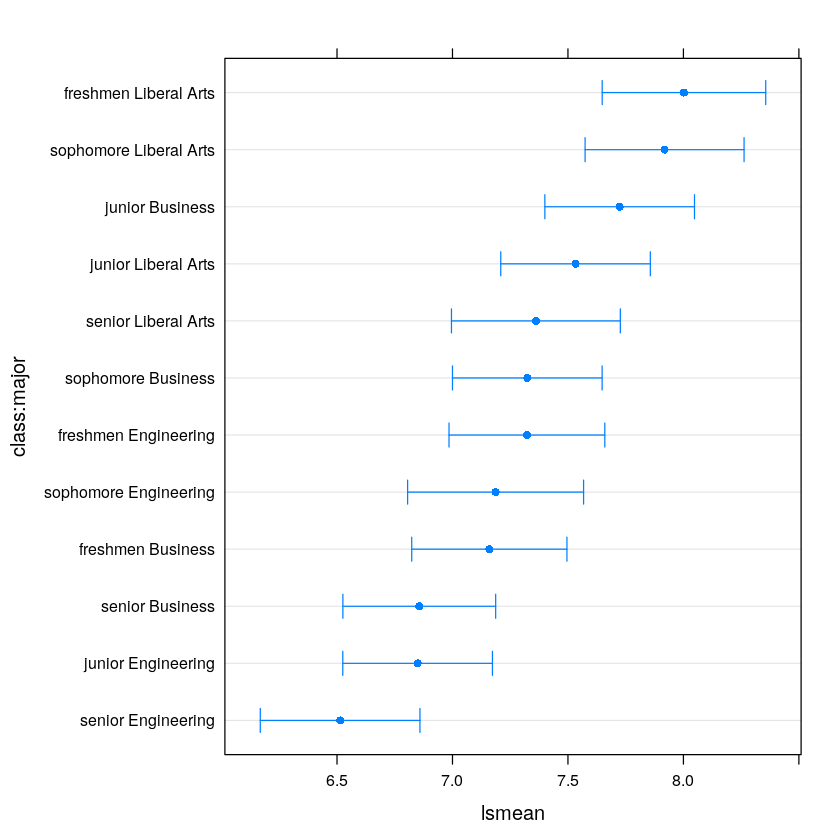
\includegraphics[height=8cm, width=10cm]{9.png}
	\end{center}
	\caption{Contrast Plot}
\end{figure}


Contrast table:

% latex table generated in R 3.5.1 by xtable 1.8-3 package
% Tue Dec  4 20:13:26 2018
\begin{table}[H]
	\centering
	\begin{tabular}{|l|r|r|r|r|l|}
		\hline\hline
		contrast & estimate & SE & df & t.ratio & p.value \\ 
		\hline
		freshmen,Business - junior,Business & -0.5644 & 0.2314 & 35 & -2.439 & 0.4084 \\ 
		freshmen,Business - senior,Business & 0.3034 & 0.2387 & 35 & 1.271 & 0.9777 \\ 
		freshmen,Business - sophomore,Business & -0.1644 & 0.2314 & 35 & -0.711 & 0.9999 \\ 
		freshmen,Business - freshmen,Engineering & -0.1628 & 0.2433 & 35 & -0.669 & 0.9999 \\ 
		freshmen,Business - junior,Engineering & 0.3106 & 0.2314 & 35 & 1.342 & 0.9670 \\ 
		freshmen,Business - senior,Engineering & 0.6461 & 0.2485 & 35 & 2.600 & 0.3174 \\ 
		freshmen,Business - sophomore,Engineering & -0.0272 & 0.2673 & 35 & -0.102 & 1.0000 \\ 
		freshmen,Business - freshmen,Liberal Arts & -0.8428 & 0.2270 & 35 & -3.713 & 0.0294 \\ 
		freshmen,Business - junior,Liberal Arts & -0.3733 & 0.2288 & 35 & -1.631 & 0.8855 \\ 
		freshmen,Business - senior,Liberal Arts & -0.2017 & 0.2288 & 35 & -0.881 & 0.9989 \\ 
		freshmen,Business - sophomore,Liberal Arts & -0.7589 & 0.2258 & 35 & -3.361 & 0.0689 \\ 
		junior,Business - senior,Business & 0.8678 & 0.2270 & 35 & 3.824 & 0.0222 \\ 
		junior,Business - sophomore,Business & 0.4000 & 0.2254 & 35 & 1.774 & 0.8205 \\ 
		junior,Business - freshmen,Engineering & 0.4017 & 0.2288 & 35 & 1.755 & 0.8300 \\ 
		junior,Business - junior,Engineering & 0.8750 & 0.2254 & 35 & 3.881 & 0.0191 \\ 
		junior,Business - senior,Engineering & 1.2106 & 0.2314 & 35 & 5.231 & 0.0004 \\ 
		junior,Business - sophomore,Engineering & 0.5372 & 0.2433 & 35 & 2.208 & 0.5548 \\ 
		junior,Business - freshmen,Liberal Arts & -0.2784 & 0.2387 & 35 & -1.166 & 0.9884 \\ 
		junior,Business - junior,Liberal Arts & 0.1911 & 0.2258 & 35 & 0.846 & 0.9993 \\ 
		junior,Business - senior,Liberal Arts & 0.3628 & 0.2433 & 35 & 1.491 & 0.9333 \\ 
		junior,Business - sophomore,Liberal Arts & -0.1945 & 0.2347 & 35 & -0.829 & 0.9994 \\
		\hline
	\end{tabular}
\end{table}


% latex table generated in R 3.5.1 by xtable 1.8-3 package
% Tue Dec  4 20:13:26 2018
\begin{table}[H]
	\centering
	\begin{tabular}{|l|r|r|r|r|l|}
		\hline
		contrast & estimate & SE & df & t.ratio & p.value \\ 
		\hline 
		senior,Business - sophomore,Business & -0.4678 & 0.2270 & 35 & -2.061 & 0.6513 \\ 
		senior,Business - freshmen,Engineering & -0.4661 & 0.2258 & 35 & -2.064 & 0.6494 \\ 
		senior,Business - junior,Engineering & 0.0072 & 0.2270 & 35 & 0.032 & 1.0000 \\ 
		senior,Business - senior,Engineering & 0.3428 & 0.2270 & 35 & 1.510 & 0.9277 \\ 
		senior,Business - sophomore,Engineering & -0.3305 & 0.2347 & 35 & -1.408 & 0.9540 \\ 
		senior,Business - freshmen,Liberal Arts & -1.1461 & 0.2485 & 35 & -4.613 & 0.0026 \\ 
		senior,Business - junior,Liberal Arts & -0.6767 & 0.2288 & 35 & -2.957 & 0.1650 \\ 
		senior,Business - senior,Liberal Arts & -0.5050 & 0.2542 & 35 & -1.986 & 0.6989 \\ 
		senior,Business - sophomore,Liberal Arts & -1.0622 & 0.2433 & 35 & -4.366 & 0.0052 \\ 
		sophomore,Business - freshmen,Engineering & 0.0017 & 0.2288 & 35 & 0.007 & 1.0000 \\ 
		sophomore,Business - junior,Engineering & 0.4750 & 0.2254 & 35 & 2.107 & 0.6215 \\ 
		sophomore,Business - senior,Engineering & 0.8106 & 0.2314 & 35 & 3.503 & 0.0493 \\ 
		sophomore,Business - sophomore,Engineering & 0.1372 & 0.2433 & 35 & 0.564 & 1.0000 \\ 
		sophomore,Business - freshmen,Liberal Arts & -0.6784 & 0.2387 & 35 & -2.842 & 0.2065 \\ 
		sophomore,Business - junior,Liberal Arts & -0.2089 & 0.2258 & 35 & -0.925 & 0.9983 \\ 
		sophomore,Business - senior,Liberal Arts & -0.0372 & 0.2433 & 35 & -0.153 & 1.0000 \\ 
		sophomore,Business - sophomore,Liberal Arts & -0.5945 & 0.2347 & 35 & -2.533 & 0.3540 \\ 
		freshmen,Engineering - junior,Engineering & 0.4733 & 0.2288 & 35 & 2.068 & 0.6465 \\ 
		freshmen,Engineering - senior,Engineering & 0.8089 & 0.2258 & 35 & 3.582 & 0.0407 \\ 
		freshmen,Engineering - sophomore,Engineering & 0.1356 & 0.2314 & 35 & 0.586 & 1.0000 \\ 
		freshmen,Engineering - freshmen,Liberal Arts & -0.6800 & 0.2542 & 35 & -2.675 & 0.2799 \\ 
		freshmen,Engineering - junior,Liberal Arts & -0.2106 & 0.2314 & 35 & -0.910 & 0.9986 \\ 
		freshmen,Engineering - senior,Liberal Arts & -0.0389 & 0.2605 & 35 & -0.149 & 1.0000 \\ 
		freshmen,Engineering - sophomore,Liberal Arts & -0.5961 & 0.2485 & 35 & -2.399 & 0.4326 \\ 
		junior,Engineering - senior,Engineering & 0.3356 & 0.2314 & 35 & 1.450 & 0.9442 \\ 
		junior,Engineering - sophomore,Engineering & -0.3378 & 0.2433 & 35 & -1.388 & 0.9583 \\ 
		junior,Engineering - freshmen,Liberal Arts & -1.1534 & 0.2387 & 35 & -4.832 & 0.0014 \\ 
		junior,Engineering - junior,Liberal Arts & -0.6839 & 0.2258 & 35 & -3.028 & 0.1428 \\ 
		junior,Engineering - senior,Liberal Arts & -0.5122 & 0.2433 & 35 & -2.106 & 0.6223 \\ 
		junior,Engineering - sophomore,Liberal Arts & -1.0695 & 0.2347 & 35 & -4.556 & 0.0030 \\ 
		senior,Engineering - sophomore,Engineering & -0.6733 & 0.2288 & 35 & -2.942 & 0.1699 \\ 
		senior,Engineering - freshmen,Liberal Arts & -1.4889 & 0.2605 & 35 & -5.715 & 0.0001 \\ 
		senior,Engineering - junior,Liberal Arts & -1.0195 & 0.2347 & 35 & -4.343 & 0.0055 \\ 
		senior,Engineering - senior,Liberal Arts & -0.8478 & 0.2673 & 35 & -3.171 & 0.1054 \\ 
		senior,Engineering - sophomore,Liberal Arts & -1.4050 & 0.2542 & 35 & -5.526 & 0.0002 \\ 
		sophomore,Engineering - freshmen,Liberal Arts & -0.8156 & 0.2822 & 35 & -2.890 & 0.1884 \\ 
		sophomore,Engineering - junior,Liberal Arts & -0.3461 & 0.2485 & 35 & -1.393 & 0.9573 \\ 
		sophomore,Engineering - senior,Liberal Arts & -0.1745 & 0.2903 & 35 & -0.601 & 1.0000 \\ 
		sophomore,Engineering - sophomore,Liberal Arts & -0.7317 & 0.2746 & 35 & -2.665 & 0.2846 \\ 
		freshmen,Liberal Arts - junior,Liberal Arts & 0.4695 & 0.2347 & 35 & 2.000 & 0.6902 \\ 
		freshmen,Liberal Arts - senior,Liberal Arts & 0.6411 & 0.2258 & 35 & 2.839 & 0.2078 \\ 
		freshmen,Liberal Arts - sophomore,Liberal Arts & 0.0839 & 0.2258 & 35 & 0.371 & 1.0000 \\ 
		junior,Liberal Arts - senior,Liberal Arts & 0.1716 & 0.2387 & 35 & 0.719 & 0.9998 \\ 
		junior,Liberal Arts - sophomore,Liberal Arts & -0.3856 & 0.2314 & 35 & -1.666 & 0.8712 \\ 
		senior,Liberal Arts - sophomore,Liberal Arts & -0.5572 & 0.2270 & 35 & -2.455 & 0.3987 \\ 
		\hline
		\multicolumn{6}{l}{{\footnotesize P value adjustment: tukey method for comparing a family of 12 estimates}}\\
	\end{tabular}
\end{table}



From the p values of contrast table of interaction terms, we could make the following conclusions:


\begin{itemize}
\item  Freshmen majoring in Business sleep significantly less than freshmen majoring in Liberal Arts;
\item  Junior majoring in Business sleep significantly more than senior majoring in Business;
\item  Junior majoring in Business sleep significantly more than junior majoring in Engineering;
\item  Junior majoring in Business sleep significantly more than senior majoring in Engineering;
\item  Senior majoring in Business sleep significantly less than freshmen majoring in Liberal Arts;
\item  Senior majoring in Business sleep significantly less than sophomore majoring in Liberal Arts;
\item  Sophomore majoring in Business sleeps significantly more than senior majoring in Engineering;
\item  Freshmen majoring in Engineering sleeps significantly more than senior majoring in Engineering;
\item  Junior,Engineering sleeps significantly less than freshmen majoring in Liberal Arts;
\item  Senior Engineering sleeps significantly less than freshmen majoring in Liberal Arts;
\item  Senior Engineering sleeps significantly less than junior majoring in Liberal Arts;
\item  Senior Engineering sleeps significantly less than sophomore majoring in Liberal Arts;
\item  No other comparisons are significantly different than zero.
\end{itemize}
\[\]

\section{Conclusion}


From the Two-Factor ANCOVA experiment conducted above to study the sleeping condition of PSU students of different class standing and different majors in November (the month before the finals) we learn that the linearity and equal slope assumption between the covariate and the response is valid and there exists an interaction effect between class standing and major. Specifically from the contrast table of the interactive combination of class standing and major , juniors and seniors who are majoring in Engineering sleep significantly less than freshmen and sophomore majoring in Liberal Arts, which confirms the speculation made in the introduction that Engineering students are more likely to shoulder more workload and that affects their sleeping conditions. 

\[\]

\section{Appendix: R Code}

\[\]

\appendix

\lstset{language=R}
\lstset{showstringspaces=false}
\lstset{frame=lines}
\lstset{caption={dataset for experiment}}
\lstset{basicstyle=\footnotesize}
\begin{lstlisting}
class=c(rep("freshmen", 12), 
	rep("sophomore", 12),
	rep("junior", 12),
	rep("senior", 12))
major=c(rep(c(rep("Engineering", 4), 
		rep("Business", 4),
		rep('Liberal Arts', 4)),
	4))
num_of_dues_per_week = c(5, 4, 6, 7,
			4, 3, 3, 5,
			2, 3, 4, 4,
			6, 5, 8, 7,
			6, 3, 4, 6,
			4, 3, 3, 4,
			4, 6, 4, 5,
			5, 4, 6, 4,
			4, 5, 5, 4,
			6, 5, 5, 7,
			6, 4, 5, 6,
			4, 2, 3, 3)
avg_sleep_hrs_per_week=c(7.1, 7.5, 7.2, 6.9, 
			7.1, 7.6, 7.4, 7.1,
			8.5, 8.3, 8.0, 8.1,
			7.0, 7.4, 6.4, 6.7,
			7.3, 8.0, 6.4, 7.5,
			8.0, 8.3, 8.2, 7.9,
			6.5, 6.6, 7.0, 7.2,
			7.5, 7.7, 7.8, 7.8,
			7.1, 7.7, 7.8, 7.6,
			6.4, 6.9, 5.9, 6.1,
			6.5, 7.3, 6.8, 6.4,
			7.4, 8.0, 7.3, 7.8)
df=data.frame(class, major, num_of_dues_per_week, avg_sleep_hrs_per_week)
\end{lstlisting}


\lstset{language=R}
\lstset{frame=lines}
\lstset{caption={Average sleeping hours per week of different majors}}
\lstset{basicstyle=\footnotesize}
\begin{lstlisting}
library(ggplot2)
library(plyr)
df_sleep <- ddply(df, .(class), transform, pos = cumsum(avg_sleep_hrs_per_week) 
						- (0.5 * avg_sleep_hrs_per_week)) 
df_sleep$class_adjusted = factor(df_sleep$class, 
			    levels=c('freshmen','sophomore', 'junior','senior'))
ggplot(df_sleep, aes(x = major, y = avg_sleep_hrs_per_week*0.25)) + 
	geom_bar(stat="identity") + 
	facet_grid(.~class_adjusted) +
	ylab('Average sleeping hours per week') + 
	xlab('Majors') +
	ggtitle('Average sleeping hours per week of different majors') +
	theme(plot.title = element_text(hjust = 0.5)) +
	theme(axis.text.x = element_text(angle = 90, size = 8))
\end{lstlisting}


\lstset{language=R}
\lstset{frame=lines}
\lstset{caption={Avgerage sleeping hours per week based on class standing and majors in PSU}}
\lstset{basicstyle=\footnotesize}
\begin{lstlisting}
ggplot(df_sleep, aes(x=major, y=avg_sleep_hrs_per_week, color=major)) +
	geom_boxplot() +
	facet_grid(vars(class_adjusted)) +
	ylab('Average sleeping hours per week') +
	ggtitle('Avgerage sleeping hours per week based on class standing and majors') +
	theme(plot.title = element_text(hjust = 0.2)) +
	ylim(min(df$avg_sleep_hrs_per_week)-0.2, 
		max(df$avg_sleep_hrs_per_week)+0.2)
\end{lstlisting}


\lstset{language=R}
\lstset{frame=lines}
\lstset{caption={Number of dues per week of different majors}}
\lstset{basicstyle=\footnotesize}
\begin{lstlisting}
df_due <- ddply(df, .(class), transform, 
		pos = cumsum(num_of_dues_per_week) - (0.5 * num_of_dues_per_week)) 
df_due$class_adjusted = factor(df_due$class,
				 levels=c('freshmen','sophomore','junior','senior'))
ggplot(df_due, aes(x = major, y = num_of_dues_per_week*0.25)) + 
	geom_bar(stat="identity") + 
	facet_grid(.~class_adjusted) +
	ylab('Average sleeping hours per week') + 
	xlab('Majors') +
	ggtitle('Number of dues per week of different majors') +
	theme(plot.title = element_text(hjust = 0.5)) +
	theme(axis.text.x = element_text(angle = 90, size = 8))
\end{lstlisting}


\lstset{language=R}
\lstset{frame=lines}
\lstset{caption={Number of dues per week based on class standing and majors in PSU}}
\lstset{basicstyle=\footnotesize}
\begin{lstlisting}
ggplot(df_due, aes(x=major, y=num_of_dues_per_week, color=major)) +
geom_boxplot() +
	facet_grid(vars(class_adjusted)) +
	ylab('Number of dues per week') +
	ggtitle('Number of dues per week based on class standing and majors') +
	theme(plot.title = element_text(hjust = 0.2)) +
	ylim(min(df$num_of_dues_per_week)-0.2, max(df$num_of_dues_per_week)+0.2)
\end{lstlisting}

\lstset{language=R}
\lstset{frame=lines}
\lstset{caption={The interaction between major/class standing and number of dues per week}}
\lstset{basicstyle=\footnotesize}
\begin{lstlisting}
mod1 <- aov(avg_sleep_hrs_per_week ~ I(num_of_dues_per_week
		-mean(num_of_dues_per_week)) + class, data = df)
mod2 <- aov(avg_sleep_hrs_per_week ~ I(num_of_dues_per_week
		-mean(num_of_dues_per_week))*class, data = df)
anova(mod1, mod2)

mod1 <- aov(avg_sleep_hrs_per_week ~ I(num_of_dues_per_week
		-mean(num_of_dues_per_week)) + major, data = df)
mod2 <- aov(avg_sleep_hrs_per_week ~ I(num_of_dues_per_week
		-mean(num_of_dues_per_week))*major, data = df)
anova(mod1, mod2)
\end{lstlisting}

\lstset{language=R}
\lstset{frame=lines}
\lstset{caption={Diagnostics of linearity and equal slopes assumptions}}
\lstset{basicstyle=\footnotesize}
\begin{lstlisting}
qplot(x = df$num_of_dues_per_week, 
		y = df$avg_sleep_hrs_per_week, 
		col = df$class,
		xlab = 'Number of dues per week',
		ylab = 'Average sleeping hours per week') + 
		geom_abline(intercept = 8.7053, 
		slope = -0.3025, 
		color="red", 
		linetype="dashed", 
		size=1)
\end{lstlisting}



\lstset{language=R}
\lstset{frame=lines}
\lstset{caption={Residuals Normality and Constance of Variance Violation Check Plot}}
\lstset{basicstyle=\footnotesize}
\begin{lstlisting}
par(mfrow=c(2,2))
plot(aov.sleep)
\end{lstlisting}


\lstset{language=R}
\lstset{frame=lines}
\lstset{caption={Interaction Plot}}
\lstset{basicstyle=\footnotesize}
\begin{lstlisting}
interaction.plot(x.factor = df$major, trace.factor = df$class,
			response = df$avg_sleep_hrs_per_week, type ="b",col = 2:3,
			xlab ="Location of StarBucks", 
			ylab ="Number of People standing in the Starbucks line",
			trace.label ="concentration")
\end{lstlisting}


\lstset{language=R}
\lstset{frame=lines}
\lstset{caption={Pairwise Differences of allinteractive  combinations}}
\lstset{basicstyle=\footnotesize}
\begin{lstlisting}
lsminter=lsmeans(aov.sleep, ~ class:major)
contrast(lsminter,method="pairwise")
contrast_inter = cld(lsminter, alpha=0.05)
plot(contrast_inter)
\end{lstlisting}

\end{document}
